\documentclass[12pt,aspectratio=169]{beamer}
\usetheme{iiasa}

\usepackage{ifthen}
\ifthenelse{\equal{\detokenize{notes}}{\jobname}}{%
\setbeameroption{show only notes}%
}{
%
}

\usepackage[
  maxnames = 1,
  style = authoryear,
  giveninits,
  terseinits,
  maxcitenames = 3,
  ]{biblatex}
\addbibresource{all.bib}

\usepackage[normalem]{ulem}

% Copied from 2020/12-03 IAMC/preamble-slides.tex %%%
\usepackage{tikz}
\usetikzlibrary{calc,scopes}

\newcommand{\side}[1]{
(0.0,#1*0.00) .. controls (0.0,#1* 0.00) and (0.4,#1*-0.04) ..
(0.4,#1*0.04) .. controls (0.4,#1* 0.11) and (0.2,#1* 0.26) ..
(0.5,#1*0.26) .. controls (0.8,#1* 0.26) and (0.6,#1* 0.11) ..
(0.6,#1*0.04) .. controls (0.6,#1*-0.04) and (1.0,#1* 0.00) ..
(1.0,#1*0.00)
}

\newcommand{\piece}[2][black]{
\begin{scope}[scale=2, shift={($(#2) - (0.25,0.48)$)}]
  \path [draw = #1, ultra thick, line cap = round]
  \side{1}  % Bottom; -1 is out, 1 is in
  [rotate around={90:(0.5,0.5)}] \side{1}    % Right
  [rotate around={180:(0.5,0.5)}] \side{-1}  % Left
  [rotate around={270:(0.5,0.5)}] \side{-1};  % Top
\end{scope}
}
%%%

\title{The MESSAGEix-GLOBIOM IAM}
\subtitle{…its development, variants, and applications—from a systems perspective}
\institute{
  Energy, Climate, and Environment (ECE) Program \\
  International Institute for Applied Systems Analysis (IIASA)}

\date{
  \texorpdfstring{Systems Modeling Summer School — Tue, 23 July 2024}%
  {2024-07-23}}

\author{\texorpdfstring{Paul Natsuo Kishimoto\scriptsize\newline
  \href{mailto:paul.kishimoto@iiasa.ac.at}%
       {\ttfamily <paul.kishimoto@iiasa.ac.at>}}%
  {Paul Natsuo Kishimoto <paul.kishimoto@iiasa.ac.at>}}

\begin{document}

\maketitle

\begin{frame}
\frametitle{Today's session}

Goal: participants see the development and some applications of MESSAGEix-GLOBIOM as one way of \structure{practicing systems modeling}.

\bigskip
\begin{description}
  \item [20’] MESSAGEix-GLOBIOM, variants, workflows, etc. (Kishimoto)
  \item [20’] Questions and open discussion.
  \item [30’] Implementing the Shared Socioeconomic Pathways (SSPs) in MESSAGEix-GLOBIOM —challenges and strategies
  \begin{description}
    \item [10’] The 2024 update of the SSPs (Fricko)
    \item [10’] Handling input data from IEA \& other sources (Joshi)
    \item [10’] Transportation (Javaid)
  \end{description}
  \item [20’] Questions and open discussion.
\end{description}

\end{frame}

\begin{frame}
\frametitle{About me}

\begin{columns}[T]
\column{0.7\textwidth}

\begin{itemize}
  \item PhD 2018 @ Engineering Systems Division, MIT.

  \begin{itemize}
    \item \href{https://web.mit.edu/fnl/volume/284/deweck.html}{Some ESD history}.
    \item Founding member of \href{https://cesun.org/about}{CESUN}.
    \item \structure{CLIOS} lens/process per Sussman \emph{et al.}:

    complex — large — interconnected — open — socio-technical systems [of systems]
    \item Credibility — salience — legitimacy of assessments per \cite{cash-2003}.
  \end{itemize}
  \item SM 2012 @ Technology Policy Program, MIT.
  \item BASc 2008 @ Engineering Science (Aerospace), U. Toronto.
\end{itemize}
\column{0.3\textwidth}
\includegraphics[width=\columnwidth]{de-weck-roos-magee-2011-cover.jpg}
\end{columns}

\smallskip
Participant in \href{https://www.ipcc.ch/report/ar6/wg3/chapter/chapter-10/}{IPCC AR6 WGIII Ch.10} — iTEM (\href{https://transportenergy.org}{transportenergy.org}) — Transport Data Commons (\href{https://transport-data.org}{transport-data.org})
\end{frame}

\begin{frame}
\frametitle{This talk}

\tableofcontents

\end{frame}

\section{MESSAGEix-GLOBIOM}

\subsection{Brief introduction}

\begin{frame}
\frametitle{“Integrated Assessment”}

MESSAGEix-GLOBIOM is a \structure{family of integrated assessment models}.

\bigskip
\begin{description}
  \item [‘integrat(ive)’] of energy, economy, environmental and other systems.
  \item [‘assessment’] mainly of large-scale changes to global systems under alternate \structure{scenarios} and \structure{constraints} that represent global policy for climate change mitigation.
  \item [models] but also a lot of machinery for input data preparation, scenario implementation, workflows output data analysis, etc.
  \item [family] there is no “[the/one] model”, but many related models with similar representation; differing in scope, resolution, etc.
\end{description}

\bigskip
\centering
\href{https://docs.messageix.org/models}{docs.messageix.org/models} —
\href{https://github.com/iiasa/message-ix-models}{github.com/iiasa/message-ix-models}

\end{frame}


\begin{frame}
\frametitle{MESSAGEix-GLOBIOM: more facts}

\begin{description}
  \item [“MESSAGE\emph{ix}”] refers to:

  \begin{itemize}
    \item \href{https://docs.messageix.org}{\ttfamily message\_ix}, an open source \emph{generic} (unparametrized) framework for models like MESSAGEix-GLOBIOM in Python, GAMS, etc. In turn \emph{‘ix’} → \texttt{ixmp}, a data storage backend and GAMS solver interface.
    \item Previous versions were “MESSAGE (V)” (5th edition), etc.
  \end{itemize}

  \item [“-GLOBIOM”] refers to a \structure{response surface-type emulator} of the GLOBIOM developed by the IIASA BNR program.
  GLOBIOM and MESSAGE are not run together (‘hard-linked’).
\end{description}

\bigskip
\begin{itemize}
  \item Dozens of contributors and users over decades of evolution.
  \item One of the category of models featured prominently in the IPCC Sixth Assessment Report (AR6), Working Group III contribution.
\end{itemize}
\end{frame}

\section{Perspectives on IAM work}

\begin{frame}
\tableofcontentscurrent
\end{frame}

\subsection{Complexity}

\begin{frame}
\frametitle{Perspectives on IAM work}

IAMs are viewed as \structure{black boxes}.
This perception is created \emph{inter alia} by choices of modelers to:

\medskip
\begin{enumerate}
  \item …\emph{not} share model code and data sufficient for genuine, scientific critique.
  \item …increase complexity of the \emph{model} in order to represent more details/disciplinary perspectives on the complex \emph{systems} within their (total) boundaries.
\end{enumerate}

\bigskip
Thankfully, tolerance for (1) is decreasing.

\medskip
But (2) tends always to get worse with time:
\begin{itemize}
  \item Model owners and collaborators are motivated to pursue novelty, increased resolution, etc.
  \item Few outside incentives for parsimony, documentation, etc.
\end{itemize}
\end{frame}

\subsection{*-disciplinarity}

\begin{frame}
\frametitle{\emph{At least} multi-disciplinary}

\includegraphics[width=\textwidth]{nastase-2017.jpg}

{\scriptsize \url{https://ian.umces.edu/blog/got-complex-problems-have-a-transdisciplinary-smoothie/}}

\begin{itemize}
  \item In order to ‘integrate’ IAMs, modelers necessarily choose (a) method(s) such as optimization…
  \item …while aware that the \structure{systems phenomena} to be captured are often the central object for entire disciplines — bodies of literature — terminology — data — methods.
\end{itemize}

\end{frame}

\subsection{Models are also software}

\begin{frame}
\frametitle{Three perspectives on models}

See \href{https://paul.kishimoto.name/2021/06/issst}{paul.kishimoto.name/2021/06/issst} for a longer talk (video \& \TeX\ slides) on this subject.

\medskip
\begin{enumerate}
  \item Knowledge objects —a representation that embodies theory.
  \item Scientific instrument —think Large Hadron Collider (LHC): expensive, crucial to build and calibrate correctly for \structure{valid results}.
  \item Software project —code, running on computers, built by teams of people in organizations.
\end{enumerate}

\bigskip
(3) is often underappreciated or brushed off—“We're not programmers, we're researchers and scientists!”—with consequences that end up undermining (2) or limiting the progress and usefulness of research.
\end{frame}

\section{Practices for valid systems research}

\begin{frame}
\tableofcontentscurrent
\end{frame}

\subsection{Software development practices}

\begin{frame}
\frametitle{Software development practices}

Learn programming basics: algorithms, data structures.

\begin{columns}
\column{0.5\textwidth}

\begin{itemize}
  \item \structure{Read} the docs to develop expertise with language and libraries.
  \item Write \structure{modular code} that follows \emph{separation of concerns}: 1 topic/task per module/file/ class/method.
  \item Write \structure{documentation}—for yourself first of all.
\end{itemize}

\column{0.5\textwidth}
\begin{itemize}
  \item Use \structure{version control} (e.g. \texttt{git}).
  \item Make code \structure{open source} on a forge like \href{https://github.com}{GitHub} or \href{https://codeberg.org}{Codeberg} from day 1.
  \item \structure{Work with others}—invite reviews of (atomic) code (changes); pair program, etc.
  \item Write \structure{tests}.
\end{itemize}
\end{columns}

\end{frame}

\begin{frame}
\frametitle{Time invested → time saved}

\centering
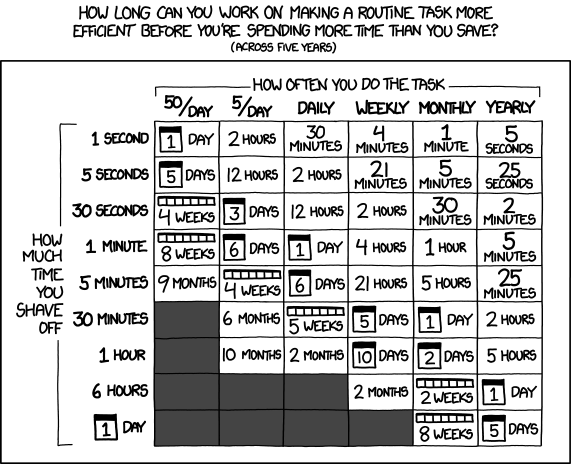
\includegraphics[height=0.8\textheight]{xkcd_1205.png}

\url{https://xkcd.com/1205/}

\end{frame}

\subsection{Data interfaces: measures and formats}

\begin{frame}
\frametitle{Be explicit about concepts \& measures}

\begin{columns}
\column{0.5\paperwidth}
\includegraphics[height=0.78\textheight]{adcock-collier-2001_f1.png}

\column{0.4\paperwidth}
{\small \fullcite{adcock-collier-2001}}

\medskip
In practice, most of the conceptualization, operationalization, and measurement for the concepts we model \structure{has already been done} by other researchers.
\end{columns}
\end{frame}


\begin{frame}[allowframebreaks]
\frametitle{Use “data interfaces”}

Specify data flows separately from methods:
\smallskip

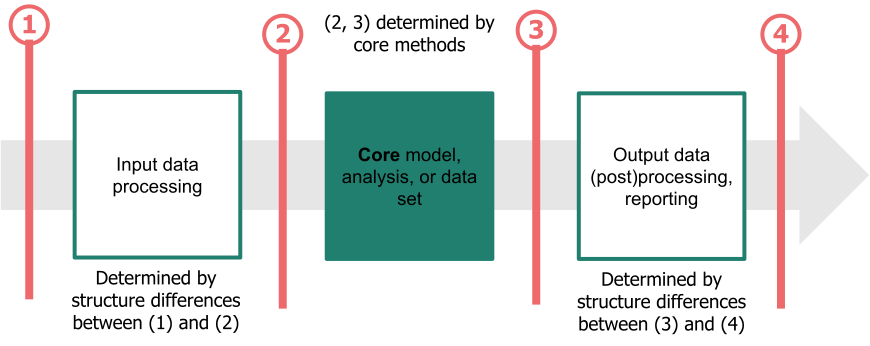
\includegraphics[width=\columnwidth]{data-stages}

These form another kind of \structure{interface} and help towards \structure{interoperability}.

\framebreak

At each interface (1) through (4) be precise about:
\begin{itemize}
  \item Background vs. systematized concepts vs. specific measures.\footcite{adcock-collier-2001}
  \item Dimensions, and the specific codes%
    \footnote{e.g. \texttt{Canada} vs. \texttt{CAN} vs. \texttt{CA}; \href{https://paul.kishimoto.name/2021/01/handling-country-codes/}{read more}.}
    used along each.
  \item Units of measurement. (Check with \href{https://pint.readthedocs.io}{Pint} or similar.)
\end{itemize}

\medskip
Treat all assumptions as input data → none in code.

\medskip
\structure{\bfseries DO NOT} invent new data formats:
\begin{itemize}
  \item Reuse existing formats and protocols for exchange

    e.g. SDMX (\href{https://sdmx.org}{1}, \href{https://sdmx1.readthedocs.io/en/latest}{2}), \href{https://www.unidata.ucar.edu/software/netcdf/}{NetCDF}, \href{https://zarr.readthedocs.io/en/stable/}{Zarr}, etc.
  \item Reuse existing (or shared) codes, categorizations, and labels

    e.g. \href{https://en.wikipedia.org/wiki/List_of_ISO_3166_country_codes}{ISO 3166-1}; \href{https://registry.sdmx.org/items/codelist.html}{SDMX global registry}.
\end{itemize}

\end{frame}

\section{More MESSAGEix-GLOBIOM}

\begin{frame}
\tableofcontentscurrent
\end{frame}

\subsection{Model variants}

\begin{frame}[allowframebreaks]
\frametitle{Model variants}

A \structure{variant} has \emph{largely similar} structure and data to the ‘base’ variant of MESSAGEix-GLOBIOM—usually with added resolution related to one or more systems. Thus far:

\medskip
\begin{description}
  \item [MESSAGEix-Nexus] of water-energy-land (→hydrology and related methods/disciplines).
  \item [MESSAGEix-Materials] detail in production, use, and recycling of materials (→industrial ecology).
  \item [MESSAGEix-Transport] detail in passenger and freight mobility (→transport research disciplines).
  \item [MESSAGEix-Buildings] energy technologies and appliances in residential and commercial buildings.
\end{description}

\medskip
Thus names like “MESSAGEix-GLOBIOM 1.1-BMT-R12”.

\framebreak

Variants are developed for \structure{targeted, in-depth investigations}, but have \emph{usage overhead} (data needs, assumptions, calibration, runtime) that may not be needed for every project.

\bigskip
Every variant \structure{corresponds to} a Python module that is used to set it up, prepare data, and post-process (report) the particular representation:
\begin{description}
  \item [MESSAGEix-Materials] → \href{https://docs.messageix.org/projects/models/en/latest/material/index.html}{\ttfamily message\_ix\_models.model.material}
  \item [MESSAGEix-Nexus] → \href{https://docs.messageix.org/projects/models/en/latest/water/index.html}{\ttfamily message\_ix\_models.model.water}
\end{description}

\bigskip
\structure{Modularity} and testing allow to compose models from variants.

\end{frame}

\begin{frame}{The ‘puzzle piece’ analogy}
\framesubtitle{Well-defined structure → interoperability}

\uncover<2>{
\begin{center}
\only<2->{
{\Large Should the components be combined like this?}

\bigskip
}
\end{center}
}

\centering
\begin{tikzpicture}[every node/.style = {text depth = 0.3ex}]
  \node (m-g) {Global};
  \piece[IIASAblue]{m-g}

  \only<1>{\coordinate (mt-pos) at ($(m-g.center) + (4, 2)$);}
  \only<2>{\coordinate (mt-pos) at ($(m-g.center) + (2, 0)$);}
  \only<3>{\coordinate (mt-pos) at ($(m-g.center) + (6, 0)$);}

  \node (mt) at (mt-pos) {Transport};
  \piece[IIASAgreen]{mt}

  \only<1>{\coordinate (bldg-pos) at ($(m-g.center) + (4, -2)$);}
  \only<2>{\coordinate (bldg-pos) at ($(m-g.center) + (4, 0)$);}
  \only<3>{\coordinate (bldg-pos) at ($(m-g.center) + (8, 0)$);}

  \node (bldg) at (bldg-pos) {Buildings};
  \piece[IIASApurple]{bldg}

  \only<1>{\coordinate (IL-pos) at ($(m-g.center) + (8, 2)$);}
  \only<2>{\coordinate (IL-pos) at ($(m-g.center) + (8, 0)$);}
  \only<3>{\coordinate (IL-pos) at ($(m-g.center) + (2, 0)$);}

  \node (IL) at (IL-pos) {Country C};
  \piece[IIASAred]{IL}

  \only<1>{\coordinate (sa-pos) at ($(m-g.center) + (8, -2)$);}
  \only<2>{\coordinate (sa-pos) at ($(m-g.center) + (6, 0)$);}
  \only<3>{\coordinate (sa-pos) at ($(m-g.center) + (4, 0)$);}

  \node (sa) at (sa-pos) {Water};
  \piece[IIASAteal]{sa}
\end{tikzpicture}

\only<2->{
\uncover<3->{
\medskip
{\centering \Large or, like this?}

\smallskip
\begin{itemize}
  \item Should this happen in only one order, or any order?
  \item How to provide a clear \& simple workflow?
  \item How to spot errors \& guide research?
\end{itemize}
}
}
\end{frame}

\subsection{Reproducible project workflows}

\begin{frame}
\frametitle{Reproducible project workflows}

Nearly every workflow for \structure{model-based research} can be broken down into the following steps:

\bigskip
\begin{enumerate}
  \item Identify \structure{what is to be represented} and desired representation.
  \item Identify a \structure{base scenario}: empty, or with some data from prior work.
  \item \structure{Build} the target scenario from the base scenario.

  May include running entire other models (“soft-linking”).
  \item \structure{Solve} the built scenario.
  \item \structure{Report} the scenario: any N-dimensional quantities, plots, or other outputs.
  \item Inspect the direct (4) and reporting (5) outputs for validity, according to some criteria.
  \item Cycle back to (1).
\end{enumerate}

\end{frame}

\begin{frame}
  \frametitle{Recap: data flows}
  \hspace*{-10mm}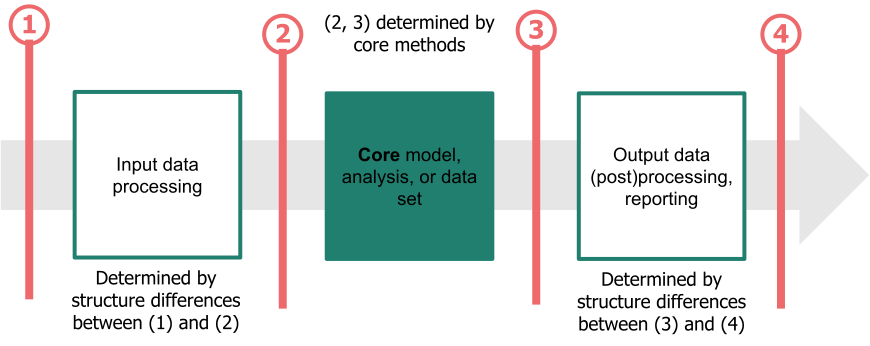
\includegraphics[width=\paperwidth]{data-stages.pdf}
\end{frame}

\begin{frame}
\frametitle{Reproducible workflows}
\framesubtitle{Some observations (1 of 2)}

\begin{columns}[T]
\column{0.2\textwidth}
\begin{enumerate}
  \item \structure{Design}.
  \item \structure{Base scenario}.
  \item \structure{Build}.
  \item \structure{Solve}.
  \item \structure{Report}.
  \item \structure{Validate}.
  \item Cycle.
\end{enumerate}

\column{0.8\textwidth}
\begin{itemize}
  \item All of these \emph{may} be done manually, but automation can help greatly.
  \item Manual steps may not be repeatable w/o clear documentation.
  \item Cost of manual steps scales if $\geq 2$ scenarios are run.
  \item (4) might be skipped—\emph{ex ante} vs. \emph{ex post} validation.
  \item Criteria (6) often vary greatly according to the intended application/RQs.
  \item Shorter cycle time → more cycles → more refined outcomes and methods (e.g. sensitivity analyses) possible.
  \item (3–5) may have sub-steps.
\end{itemize}

\end{columns}
\end{frame}

\begin{frame}
\frametitle{Reproducible workflows}
\framesubtitle{Further observations (2 of 2)}

\begin{columns}[T]
\column{0.2\textwidth}
\begin{enumerate}
  \item \structure{Design}.
  \item \structure{Base scenario}.
  \item \structure{Build}.
  \item \structure{Solve}.
  \item \structure{Report}.
  \item \structure{Validate}.
  \item Cycle.
\end{enumerate}

\column{0.8\textwidth}
Often we want to \structure{chain}, \structure{nest}, or \structure{merge} workflows.

\smallskip
Ex. 1: combine ‘build’ substeps from MESSAGEix-Transport and a workflow that sets up a specific (but generic) climate policy.

\smallskip
Ex. 2: combine ‘build’ substeps from the MESSAGEix-Transport, -Buildings, and -Materials workflows to produce a "B-M-T" target scenario.

\smallskip
Ex. 3: combine ‘report’ substeps for MESSAGEix-Transport and the base M-G model.

\smallskip
Ex. 4: ‘build’ the policy parametrization of one scenario based on the ‘solved’ or ‘reported’ outcome of another.
\end{columns}
\end{frame}

\begin{frame}
\frametitle{Repeatable → reproducible}

We use the concepts of a chain of nodes (scenarios) and edges (workflow steps) at a high level of abstraction.
Implemented in the \texttt{message-ix-models} Python package; see docs on \href{https://docs.messageix.org/projects/models/en/latest/api/workflow.html}{“Multi-scenario workflows”}.

\bigskip
Define atomic workflow steps → compose workflows using these.

\bigskip
Provide a \structure{command-line interface} to run entire workflows or portions; other tools to visualize, log, diagnose.

\bigskip
Define the methods for projects by reference to repeatable commands: “Using version 2024.7.23 of \texttt{message-ix-models} [and associated dependencies/input data], run the command:

\texttt{mix-models --url="..." ssp run --options=A,B,Z --node=R12 --go}”
\end{frame}

\subsection{Misc. goodies}

\begin{frame}
\frametitle{Miscellaneous goodies}

\begin{itemize}
  \item Our documentation contains lists of codes for \href{https://docs.messageix.org/projects/models/en/latest/pkg-data/node.html}{spatial units}, \href{https://docs.messageix.org/projects/models/en/latest/pkg-data/year.html}{time periods}, \href{https://docs.messageix.org/projects/models/en/latest/pkg-data/codelists.html}{technologies and more} used in the model.
  \item We have \href{https://github.com/iiasa/message-ix-models/actions}{automated test workflows} that run on (daily) schedules and confirm model-building codes work with latest versions of upstream data and software.
  \item Model snapshot data are published to Zenodo (e.g. \href{https://doi.org/10.5271/zenodo.10514052}{doi: 10.5271/zenodo.10514052}); the code can automatically fetch, unpack, load, solve, and report these (\href{https://docs.messageix.org/projects/models/en/latest/api/model-snapshot.html}{docs}).
  \item We use \href{https://github.com/iiasa/message_ix/discussions}{GitHub discussions}, Slack, and other tools to interact with a wide variety of users.
\end{itemize}

\end{frame}

\section*{Discussion}

\begin{frame}
\frametitle{Discussion (20’)}

We could cover:

\medskip
\begin{itemize}
  \item More detail/rationale on any of the above points, acronyms, concepts.
  \item Same concepts you've seen expressed elsewhere with different names.
  \item Other examples of models, tools, etc. that were useful because of similar practices.
  \item Examples of failures/missed opportunities due to poor model reusability or data incompatibility.
  \item “Capacity building” and open science: is systems modeling an ivory-tower pursuit, or a means to solving real-world problems?

\end{itemize}
\end{frame}

\begin{frame}[c,plain]
  \vfill
  {\centering \Huge \structure{Thank you!}}

  \vfill
  \textcopyright\ Copyright 2024 Paul Natsuo Kishimoto.

  \raisebox{-.1\height}{%
  \includegraphics[height=1em]{cc.pdf}%
  \includegraphics[height=1em]{cc-by.pdf}%
  \includegraphics[height=1em]{cc-sa.pdf}%
  }
  Licensed \href{https://creativecommons.org/licenses/by-sa/4.0/}{Creative Commons BY-SA 4.0}

  \TeX\ source at \url{https://github.com/khaeru/doc/}
\end{frame}

\appendix

\begin{frame}
\frametitle{References}

\nocite{de-weck-roos-magee-2011}

\printbibliography[heading=none]

\end{frame}

\end{document}
